\chapter{Estado del arte}

Este capítulo ofrece una visión actualizada de los recursos, tecnologías y enfoques más relevantes para la gestión y análisis de datos clínicos. Se abordan las principales bases de datos abiertas, los modelos de almacenamiento y consulta, las arquitecturas de software más empleadas, las herramientas de visualización y el impacto de la Inteligencia Artificial en el ámbito sanitario, situando el proyecto dentro del contexto de la innovación digital en salud.

%\section{El Movimiento hacia la Ciencia Abierta en la Investigación Médica}
\section{Ciencia abierta y bases de datos clínicas}

En las últimas décadas se ha consolidado un movimiento hacia los datos clínicos abiertos, promoviendo la disponibilidad de bases de datos sanitarias para la comunidad investigadora. La idea de ciencia abierta sostiene que la libre disponibilidad de datos y códigos favorece la transparencia, la reproducibilidad y la colaboración en la investigación biomédica \cite{Lvovs2025_balancing}. Sin embargo, históricamente los datos clínicos han estado protegidos en archivos hospitalarios, difíciles de acceder por razones legales, éticas y técnicas. En respuesta, iniciativas académicas y gubernamentales han impulsado la creación de conjuntos de datos clínicos de acceso abierto, debidamente anonimizados, que permiten a investigadores de todo el mundo analizar información real de pacientes sin vulnerar la privacidad. Estos recursos han transformado la investigación médica al reducir barreras de acceso y fomentar prácticas reproducibles en análisis de datos sanitarios

\newpage
Los datos clínicos se pueden clasificar en cuatro grandes modalidades complementarias:


(i) \emph{Señales fisiológicas de alta frecuencia.} Series temporales de ECG, presión arterial invasiva, fotopletismografía o EEG. Podemos destacar la clásica MIT-BIH Arrhythmia Database (1980), patrón de referencia para algoritmos de ECG \cite{Impact_MIT-BIH}; el MIMIC Waveform Database, que enlaza miles de horas de señales con los datos clínicos de MIMIC \cite{Moody2022_MIMICIVWaveform}; y HiRID, con 712 variables registradas cada dos minutos en más de 30 000 estancias UCI \cite{Faltys2021HiRID}.

(ii) \emph{Imágenes médicas con anotaciones diagnósticas.}  Abarcan radiografías, TC, RM, PET e incluso histopatología digital, cada una acompañada de etiquetas o informes de hallazgo.  Las bases más usadas en radiología son ChestXray14 y CheXpert, ambas con cientos de miles de radiografías torácicas etiquetadas para patologías pulmonares \cite{irvin2019chexpertlargechestradiograph}, y MIMIC-CXR por parte de la familia MIMIC \cite{Johnson2019_MIMICCXR}.  En oncología destacan las colecciones TCGA/TCIA \cite{TCGA,Clark2013_TCIA}, y en neuroimagen la iniciativa ADNI \cite{Petersen2010_ADNI}.  Estos recursos posibilitan evaluar modelos de visión computacional con criterios homogéneos.

(iii) \emph{Texto clínico desidentificado.}  Incluye notas de evolución, informes radiológicos, resúmenes de alta, entre otros.  Representa alrededor del 80 \% de la información clínica, pero su liberación es más compleja por contener PHI (Protected Health Information).  Los desafíos i2b2/n2c2, pioneros al proveer corpora anonimizados, constituyen la plataforma estándar para comparar sistemas de procesamiento del lenguaje natural médico \cite{n2c2}.  El ecosistema MIMIC también complementa este dominio con millones de notas clínicas \cite{Johnson2023_MIMICIVNote}. 

(iv) \emph{Datos estructurados de historias clínicas electrónicas (EHR).}  Comprenden tablas con demografía, diagnósticos (ICD-9/10), procedimientos, resultados de laboratorio, medicación y constantes vitales.  Son la base de estudios epidemiológicos y de la construcción de modelos pronósticos.  Entre los conjuntos abiertos más influyentes figuran NHANES \cite{NHANES}, UK Biobank \cite{Sudlow2015_UKBiobank}, eICU \cite{Pollard2018} y, sobre todo, la serie MIMIC en la que se enfoca este trabajo.

Desde 1999 PhysioNet \cite{PhysioNet_paper} estableció un marco seguro y reproducible para compartir todo tipo de registros hospitalarios.  Bajo ese paraguas nació el ecosistema MIMIC: la primera versión (1996) contenía 90 pacientes UCI \cite{Moody1996_MIMIC}; MIMIC-II (2011) multiplicó tamaño y variables al extraer directamente de los sistemas clínicos \cite{Saeed2011_MIMICII}; MIMIC-III (2015) superó los 40 000 pacientes y se convirtió en la referencia mundial \cite{MIMICIII_paper}; MIMIC-IV \cite{MIMICIV_paper} amplía y moderniza el conjunto.  Esta trayectoria demuestra cómo los EHR han pasado a ser un recurso científico global, permitiendo investigar la fisiopatología crítica con una profundidad antes impensable.

\begin{figure}[ht]
    \centering
    \fbox{
\includegraphics[width=0.4\textwidth]{imagenes/physionet-logo.png}}
    %
\includegraphics[width=0.4\textwidth]{imagenes/physionet-logo.png}
    \caption{Logo de PhysioNet.}
\end{figure}

\newpage
En conjunto, el panorama de datos clínicos abiertos ofrece múltiples alternativas, pero MIMIC-IV destaca como la más idónea para este trabajo: combina un gran volumen de datos reciente, buena documentación, y módulos complementarios. Sobre esta base, el proyecto diseñará una plataforma que haga de este conjunto de datos una fuente accesible de conocimiento, alineada con los principios de ciencia abierta.


%\section{Tecnologías para la Gestión y Almacenamiento de Datos Sanitarios}
\section{Tecnologías de Gestión y Almacenamiento de Datos Sanitarios}




En el plano tecnológico, la forma de almacenar y consultar la información marca las posibilidades reales de análisis. De forma general, los sistemas de gestión de bases de datos se dividen en dos grandes familias: relacionales y no relacionales. Las del primer grupo organizan la información en tablas de filas y columnas conectadas por claves y se consultan con SQL, siendo las más usadas MySQL, PostgreSQL, Oracle y SQL Server.  Las no relacionales, llamadas NoSQL, almacenan los datos como documentos, pares clave-valor, columnas o grafos y permiten esquemas flexibles y escalado horizontal; las más populares son MongoDB y Couchbase en la categoría de documentos, Cassandra en column-family, Redis en clave-valor y Neo4j en grafos \cite{DBEngines2025}.

\begin{figure}[H]
    \centering
    \fbox{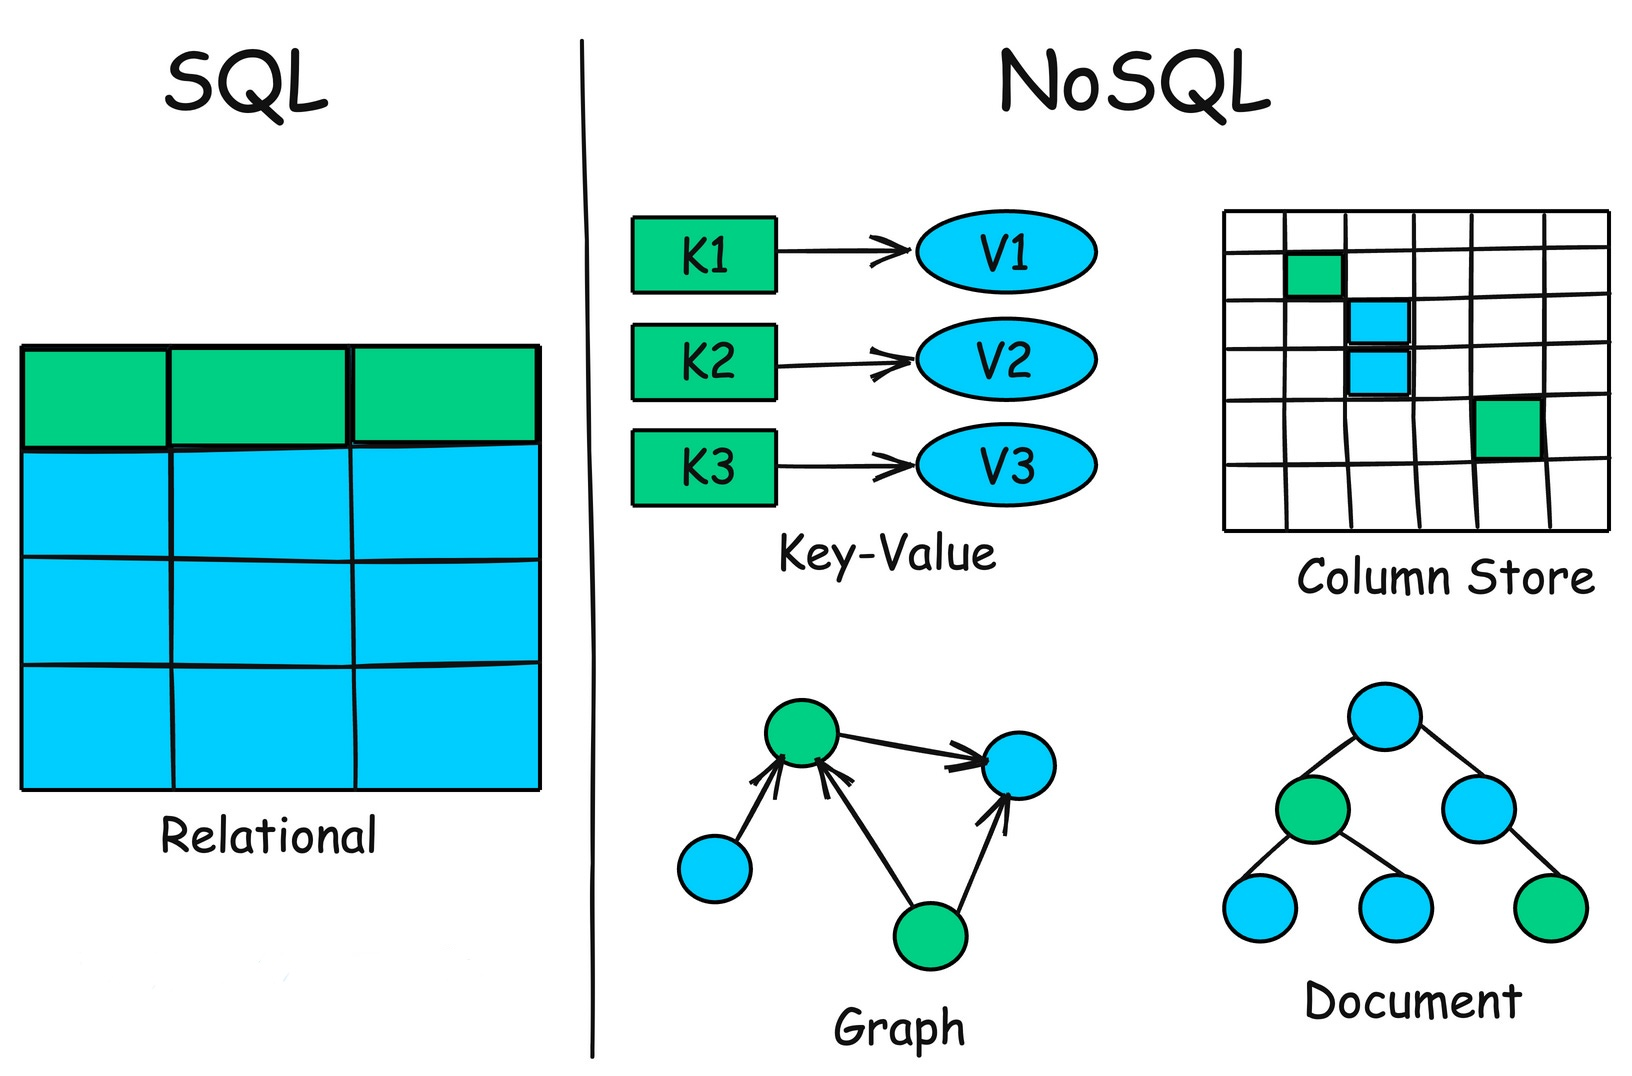
\includegraphics[width=0.75\textwidth]{imagenes/sqlvsnosql.jpg}}
    %
\includegraphics[width=0.4\textwidth]{imagenes/physionet-logo.png}
    \caption{SQL vs NoSQL \cite{sqlvsnosqlfoto}.}
\end{figure}


En el ámbito sanitario la mayoría de los sistemas de historia clínica electrónica se ha construido sobre gestores relacionales porque los registros se modelan de forma natural en tablas normalizadas y el lenguaje SQL facilita auditoría y trazabilidad.  Sin embargo, los hospitales también generan notas de texto libre, señales continuas, imágenes y estructuras jerárquicas; ello ha impulsado el uso de bases documentales y de grafos, que aceptan datos heterogéneos y simplifican la ingesta sin migraciones de esquema cada vez que aparece un nuevo campo \cite{GAMAL2021103670,MongoFHIR}.

%A pesar de que MIMIC-IV se distribuye en un esquema relacional, para este proyecto cargaremos el conjunto en MongoDB. Este modelo documental nos permite agrupar los datos que se deseen en un único documento anidado, elimina la necesidad de combinar una veintena de tablas con uniones complejas y responde con menor latencia a las búsquedas interactivas que planteará el usuario desde la interfaz web.  Además, nos ofrece flexibilidad y escalabilidad si en el futuro se desea incorporar señales o imágenes, de modo que se adapta mejor a la naturaleza exploratoria y multimodal de nuestra aplicación.


%\section{Arquitecturas de Software y el Stack Tecnológico Web}
\section{Arquitecturas de Software y  Stack Web}

La evolución del desarrollo de software ha experimentado una transformación radical desde las aplicaciones de escritorio tradicionales hacia ecosistemas web distribuidos. En los años 90, la Web se caracterizaba por páginas estáticas servidas directamente desde servidores, pero la creciente demanda de interactividad y funcionalidad dinámica impulsó el desarrollo de tecnologías como CGI, PHP y posteriormente frameworks más sofisticados \cite{Ritesh2023_WebEvolution}. Esta evolución culminó en las aplicaciones web contemporáneas, que se fundamentan en la arquitectura cliente-servidor, donde el frontend ejecutado en el navegador del usuario se comunica con un backend que procesa la lógica y gestiona el acceso a los datos \cite{Nyabuto2024_ClientServer}. Esta separación de responsabilidades permite que cada componente evolucione independientemente, facilita el mantenimiento del código y posibilita la escalabilidad según las necesidades específicas de cada capa. En el contexto de aplicaciones de análisis de datos como la que nos ocupa, esta arquitectura resulta especialmente ventajosa al permitir que el procesamiento computacionalmente intensivo se realice en el servidor mientras el cliente se centra en la presentación interactiva de los resultados.

%begin{figure}[H]
%    \centering
%    \fbox{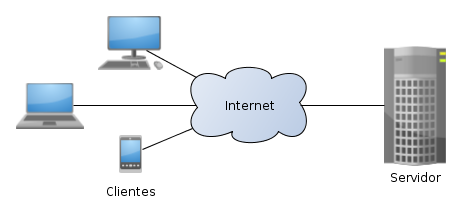
\includegraphics[width=0.75\textwidth]{imagenes/Cliente-Servidor.png}}
%    %
\includegraphics[width=0.4\textwidth]{imagenes/physionet-logo.png}
%    \caption{Diagrama cliente-servidor \cite{clienteservidorfoto}.}
%\end{figure}

\begin{figure}[H]
    \centering
    \fbox{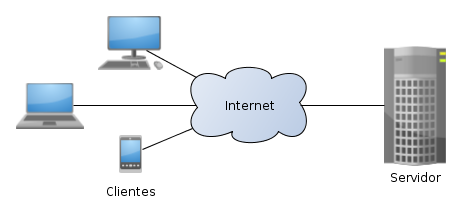
\includegraphics[width=0.85\textwidth]{imagenes/Cliente-Servidor.png}}
    %
\includegraphics[width=0.4\textwidth]{imagenes/physionet-logo.png}
    \caption{Diagrama cliente-servidor \cite{clienteservidorfoto}.}
\end{figure}




En cuanto a las tecnologías de servidor, existe un amplio abanico de alternativas consolidadas, cada una con fortalezas específicas según el contexto de aplicación. Node.js con frameworks como Express o Fastify permite utilizar JavaScript en el servidor, facilitando el desarrollo full-stack y ofreciendo excelente rendimiento para aplicaciones I/O intensivas. Python, con opciones como Django, Flask y FastAPI, destaca en proyectos que requieren análisis de datos o integración con librerías científicas \cite{Castro2023_PythonDataScience}. Java con Spring Boot sigue siendo una opción robusta para aplicaciones empresariales de gran escala, mientras que lenguajes como Go y Rust están ganando adopción por su rendimiento superior en sistemas distribuidos. %En el contexto de este proyecto, donde el procesamiento de datos biomédicos y la futura integración de modelos de inteligencia artificial son requisitos centrales, se ha optado por FastAPI con Python, aprovechando tanto su ecosistema maduro para análisis de datos como su capacidad para generar APIs modernas y eficientes.

Por otro lado, las tecnologías frontend han experimentado una evolución significativa desde las aplicaciones de página única (SPA) hacia enfoques más sofisticados que combinan diferentes estrategias de renderizado. Los frameworks principales \cite{Swacha2023_WebFrameworks} incluyen React, que ofrece un ecosistema maduro y flexible basado en componentes; Vue.js, conocido por su curva de aprendizaje suave y documentación excelente; y Angular, que proporciona un framework completo con opiniones definidas para aplicaciones empresariales. Paralelamente, han surgido meta-frameworks como Next.js, Nuxt.js y SvelteKit que extienden estos frameworks base con capacidades de renderizado del lado del servidor (SSR), generación de sitios estáticos (SSG) y optimizaciones automáticas. %Para este proyecto se ha seleccionado Next.js sobre React, desplegado en Vercel, una combinación que permite aprovechar tanto el renderizado híbrido para optimizar el rendimiento del análisis y visualización de datos.

\begin{figure}[H]
\centering
\fbox{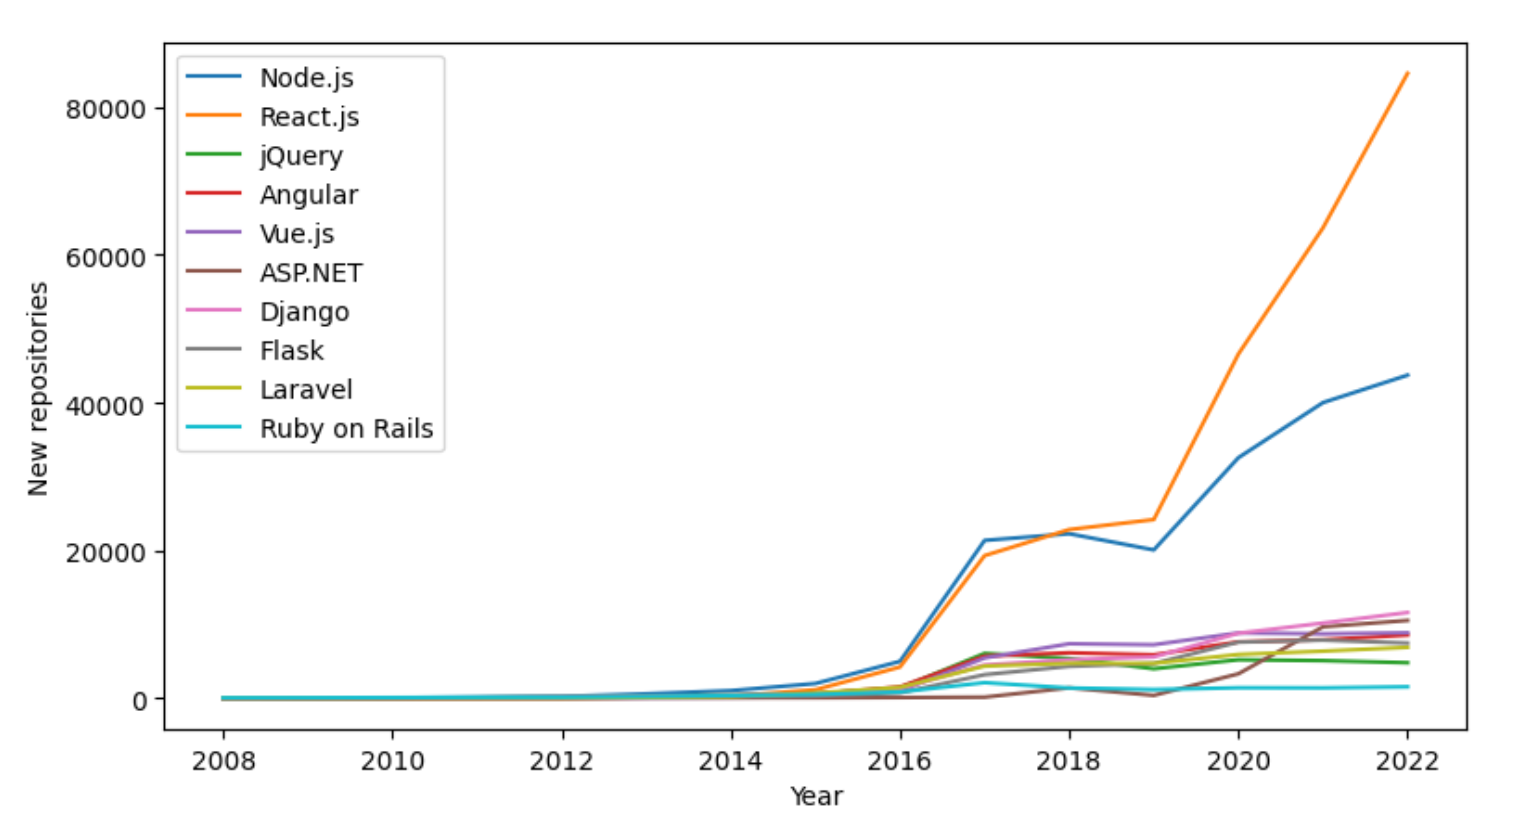
\includegraphics[width=1\textwidth]{imagenes/grafica_frameworks.png}}
%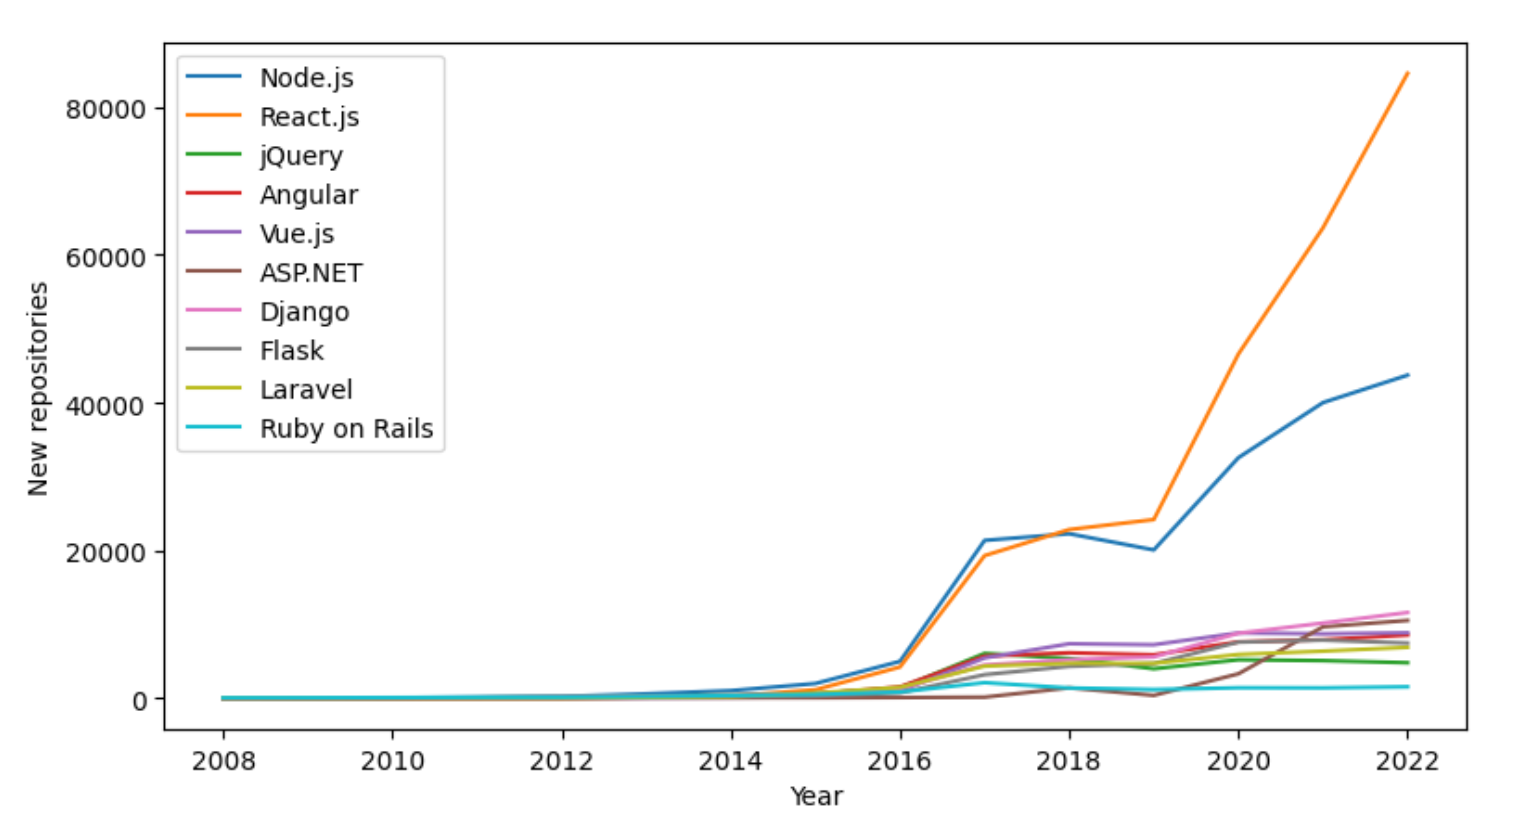
\includegraphics[width=\textwidth]{imagenes/grafica_frameworks.png}
\caption{Evolución de la popularidad de frameworks web según el número de repositorios creados anualmente en GitHub \cite{Swacha2023_WebFrameworks}.}
\label{fig:frameworks_github}
\end{figure}



%\section{Herramientas y Técnicas de Visualización Interactiva de Datos}
\section{Herramientas de Visualización Interactiva de Datos}

Para la visualización de datos en aplicaciones web existen principalmente dos tipos de herramientas: plataformas de business intelligence (Tableau, Power BI, Metabase) y librerías de programación para desarrolladores. Las plataformas de business intelligence permiten a usuarios no técnicos explorar y analizar datos mediante interfaces gráficas intuitivas, facilitando la creación de dashboards interactivos y la generación de informes sin necesidad de programar. Sin embargo, estas plataformas suelen estar más orientadas al análisis empresarial general y pueden presentar limitaciones cuando se requiere una personalización avanzada o la integración directa con aplicaciones web personalizadas.

Por otro lado, las librerías de programación ofrecen a los desarrolladores un control total sobre la visualización y permiten crear gráficos completamente adaptados a las necesidades de cada proyecto. Entre las librerías más utilizadas para Javascript destacan D3, Chart.js, Plotly.js y ECharts, por nombrar algunas, aunque el ecosistema es muy amplio y en constante evolución \cite{Monterail2024_JSViz}. Estas herramientas permiten desde la creación de gráficos básicos hasta visualizaciones interactivas complejas, integrándose perfectamente en aplicaciones web modernas y proporcionando una experiencia de usuario más dinámica y personalizada.


%En el contexto de este proyecto, se ha optado por usar dos librerías distintas, dependiendo de la complejidad del gráfico, pero que son desarrolladas por la misma compañía denominada Observable \cite{observable}. Se utiliza D3 \cite{d3} para visualizaciones altamente personalizadas que requieren máximo control granular sobre cada elemento gráfico, lo que resulta especialmente útil para representar datos clínicos complejos o relaciones no convencionales. Por otro lado, se reserva Plot \cite{observableplot} para las visualizaciones más sencillas y habituales, aprovechando sus soluciones preestablecidas que aceleran el desarrollo y reducen la carga de trabajo en la implementación. Esta combinación permite mantener un enfoque progresivo en complejidad, acelerando la rapidez de implementación y manteniendo una coherencia estética y técnica al permanecer dentro del mismo ecosistema de herramientas.

\begin{figure}[H]
    \centering    \fbox{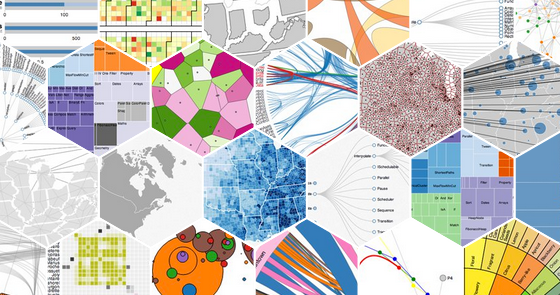
\includegraphics[width=0.85\textwidth]{imagenes/d3.png}}
    %
\includegraphics[width=0.4\textwidth]{imagenes/physionet-logo.png}
    \caption{Visualizaciones realizadas con D3 \cite{d3foto}.}
\end{figure}



%\section{Aplicaciones de Inteligencia Artificial en el Análisis Clínico}
\section{Grandes Modelos de Lenguaje (LLM) en Medicina}

Los grandes modelos de lenguaje basados en Transformers han irrumpido en la práctica clínica porque ofrecen comprensión contextual y generación de texto con una fluidez cercana a la humana. A diferencia de los modelos supervisados tradicionales, los LLMs aprenden a partir de preentrenamiento masivo y pueden adaptarse con pocos ejemplos, rasgo que resulta valioso cuando los conjuntos de datos clínicos etiquetados son escasos. Este cambio de paradigma coincide con la disponibilidad de texto sanitario desidentificado, lo que ha catalizado su adopción en investigación biomédica.


Después de la aparición de modelos generalistas como GPT-3 \cite{Brown2020GPT3} se publicaron variantes especializadas en biomedicina entrenadas sobre literatura científica y notas de pacientes. ClinicalBERT \cite{Boag2020_ClinicalBERT} y BioGPT \cite{Lee2020_BioBERT} demostraron que un preentrenamiento adicional en dominio mejora la extracción de entidades médicas y la clasificación de relaciones. Más recientemente, GatorTron \cite{Yang2022_GatorTron}, Med-PaLM 2 \cite{Singhal2023_MedPaLM2} y Llama-Med \cite{Xie2024_MeLLaMA} ampliaron el tamaño de parámetros y el repertorio de instrucciones clínicas, acercándose al rendimiento de especialistas humanos en tareas de respuesta a preguntas complejas.

La integración de estos modelos en sistemas hospitalarios adopta varias estrategias. La más extendida es la generación aumentada por recuperación, en la que el LLM consulta primero una base indexada de guías clínicas o registros electrónicos y después compone la respuesta citando la información recuperada \cite{RAGSurvey2023}. Otra línea es el ajuste fino con instrucciones específicas que enseñan al modelo a traducir preguntas en lenguaje natural a consultas estructuradas sobre bases de datos; ChatEHR es un ejemplo que opera sobre historiales electrónicos \cite{Stanford2025_ChatEHR}. El Model Context Protocol (MCP) propone una capa intermedia para que el modelo invoque herramientas, agentes o bases de datos de forma segura, lo que facilita operaciones más complejas que la simple generación de texto \cite{AnthropicMCP2024}.

El éxito de estas técnicas depende de corpus clínicos abiertos que permitan la adaptación en dominio. Las notas de MIMIC-III y MIMIC-IV \cite{Johnson2023_MIMICIVNote}, los desafíos i2b2/n2c2 \cite{n2c2} (ya mencionadas anteriormente) y colecciones de pregunta–respuesta como PubMedQA \cite{Jin2019_PubMedQA} y MedQA \cite{Jin2020_MedQA} constituyen hoy los pilares para la evaluación reproducible de PLN médico. No obstante, la sensibilidad de la información obliga a procesos de anonimización rigurosos y a la aplicación de licencias restrictivas.

A pesar de su potencial, los LLMs plantean riesgos significativos. Pueden generar afirmaciones verosímiles pero erróneas, lo que compromete la seguridad clínica; además, arrastran sesgos demográficos si los datos de entrenamiento son incompletos y pueden filtrar información protegida si no se controla el \textit{fine-tuning}. La comunidad trabaja en métricas de evaluación específicas y en detectores de alucinaciones, pero todavía no existe un consenso regulatorio sobre su despliegue en entornos asistenciales \cite{Bommasani2022_FoundationModels}. Estos retos marcan la agenda de investigación actual y condicionan las directrices éticas para cualquier sistema que integre LLMs con datos reales de pacientes.



\section{Aplicaciones existentes similares}\

En el ámbito hospitalario existen numerosas soluciones comerciales consolidadas para la gestión y análisis de datos clínicos. Sistemas como Epic Systems integran módulos de visualización de indicadores, generación de informes y cuadros de mando en tiempo real, con funcionalidades que incluyen predicción de riesgos, alertas clínicas y exploración de cohortes directamente sobre la historia clínica electrónica \cite{Epic}. Este tipo de plataformas están diseñadas para su uso en entornos de producción con pacientes reales y representan el estándar en hospitales de gran escala, aunque se trata de soluciones cerradas y de acceso restringido al entorno clínico que las contrata.

En contraste, las opciones de código abierto para la visualización de datos médicos son mucho más limitadas en número y funcionalidades. LinkR es un proyecto reciente orientado a la exploración y visualización de datos clínicos siguiendo el estándar OMOP \cite{linkR}. Como otro ejemplo, Metriport a pesar de no ser su función principal, permite visualizar los datos clínicos, usando IA para resumir los historiales clínicos de los pacientes, y también posee una capa open source \cite{metriport}. En general, se ha encontrado que son muy escasos los recursos abiertos, actualizados y en mantenimiento en este ambito.


En cuanto a la exploración específica de MIMIC-IV, no se han identificado plataformas web abiertas que ofrezcan de forma nativa una visualización interactiva del conjunto de datos. La aproximación más utilizada en la literatura consiste en cargar el conjunto de datos en entornos analíticos en la nube, como Google BigQuery combinado con Looker Studio, lo que permite construir paneles y gráficos sin necesidad de programación \cite{bigquery_mimic}. Otra alternativa es la conversión de los datos al estándar OMOP, lo que hace posible su explotación a través de herramientas como OHDSI Atlas, que incluye funcionalidades de análisis de cohortes y visualización \cite{OHDSI_Atlas, MIMICIV_OMOP_Demo}. No obstante, estas opciones requieren configuraciones avanzadas y no existen soluciones abiertas, listas para usar, que faciliten directamente la exploración gráfica de MIMIC-IV a investigadores sin conocimientos técnicos.



\section{Síntesis y foco del presente TFG}

El repaso realizado muestra un contraste evidente entre las soluciones comerciales y el panorama abierto. En el entorno hospitalario, las grandes plataformas de EHR concentran el grueso de la innovación en visualización y análisis de datos clínicos. Se trata de sistemas completos, diseñados para la práctica asistencial diaria, con interfaces pulidas y funcionalidades avanzadas de predicción y apoyo a la decisión clínica. Sin embargo, son soluciones cerradas y restringidas a los centros que las contratan.

En el ámbito open source, la situación es distinta. Existen numerosas bases de datos abiertas que han impulsado la investigación biomédica en todo el mundo. Sin embargo, las herramientas disponibles para explorarlas son menos accesibles para usuarios sin experiencia técnica. Los investigadores suelen recurrir a consultas SQL, entornos estadísticos o integraciones complejas con plataformas de terceros, lo que limita su aprovechamiento por parte de perfiles clínicos sin formación tecnológica. Las interfaces gráficas abiertas y mantenidas son escasas y, cuando existen, tienden a estar más orientadas a la investigación metodológica que a la usabilidad clínica.

En este contexto se sitúa el presente trabajo. El objetivo no es competir con los sistemas hospitalarios consolidados, sino plantear un prototipo que sirva como demostración de cómo un conjunto de datos abierto como MIMIC-IV puede hacerse accesible mediante una plataforma web sencilla de usar. El sistema combina visualización interactiva con integración de modelos de inteligencia artificial recientes, ilustrando cómo los profesionales sin conocimientos técnicos podrían extraer valor de bases de datos clínicas abiertas. De este modo, el proyecto se posiciona como un puente entre la abundancia de datos disponibles y la carencia de interfaces accesibles para su exploración.

